\chapter{Evaluation}\label{chap:evaluation}

This chapter presents the findings and results from the experiments outlined in the specification \& design chapter (\ref{chap:specification-design}) as well as the implementation chapter (\ref{chap:implementation}). We evaluate the classifiers' performance, first on their respective datasets, then on the other dataset to assess transferability. We then explore the relevant SHAP values for each experiment, reasoning about the importance of the features in the models.

\section{Performance Evaluation}\label{sec:performance-evaluation}

As described in section (\ref{sec:TransferabilityEvaluation}), the classifiers are evaluated on their respective datasets and then on the other dataset to assess transferability. The performance metrics tested include accuracy, precision, recall, and F1 score. The results are presented in Figures~\ref{fig:classifier_performance_same_dataset} and~\ref{fig:classifier_performance_across_dataset}.

\subsection{Performance on the Same Dataset}\label{subsec:performance-same-dataset}

\begin{figure}[H]
\centering
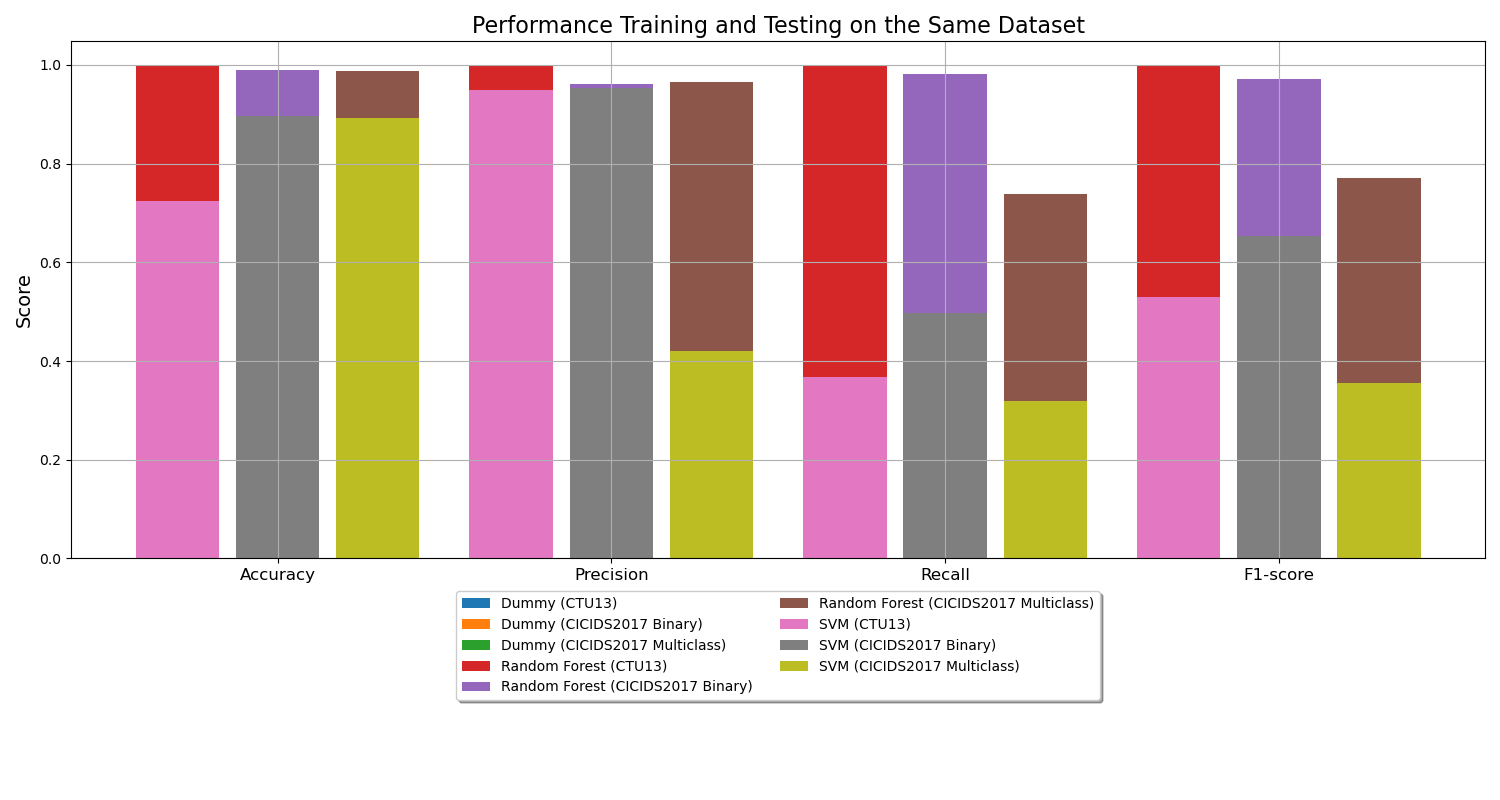
\includegraphics[width=\textwidth]{img/Classifier_Performance_Same_Dataset.png}
\caption{Classifiers' performance on the same datasets.}\label{fig:classifier_performance_same_dataset}
\end{figure}

When testing the classifiers' performance on the same dataset, they were trained on; we note some promising results. The Random Forest model achieves an accuracy of 0.99, precision of 0.99, recall of 0.99, and F1 score of 0.99 on the CTU13 dataset. The model also performs well on the CICIDS2017 dataset, with an accuracy of 0.99, precision of 0.96, recall of 0.98, and F1 score of 0.97 when focusing on binary classification. These results indicate that the classifiers detect malicious traffic on their respective datasets effectively.

In the multi-class classification, the Random Forest model achieves a respectable F1 score of 0.78, with an accuracy of 0.99, precision of 0.90, and recall of 0.76. While these scores would likely need to be higher to deploy the multi-class model in a real-world scenario, they outperform the dummy classifier's baseline score of 0.66, proving that the model learns from the data.

When considering the performance of the classifiers on the same dataset, all three Random Forest classifiers outperform the dummy classifier, showing that, at least in the context of the datasets used, the classifiers are learning from the data and making accurate predictions.

The SVM classifier's performance was worse than the Random Forest's; it also ended up being worse than the dummy classifier's performance. The SVM classifier trained on CTU13 achieves an accuracy of 0.73, precision of 0.96, recall of 0.37, and an F1 score of 0.53 when tested on CTU13. The binary model trained on CICIDS2017 achieves an accuracy of 0.73, precision of 0.96, recall of 0.37, and an F1 score of 0.65 when tested on CICIDS2017. The multi-class SVM model trained on CICIDS2017 achieves an accuracy of 0.89, precision of 0.42, recall of 0.32, and an F1 score of 0.35 when tested on CICIDS2017, indicating that the SVM classifiers are not as effective as the Random Forest classifiers at detecting malicious traffic on the datasets used, at least with the current implementation (we will discuss improvements in the conclusion chapter\ref{chap:conclusion-future-work}).

\subsection{Performance on Different Datasets}\label{subsec:performance-different-dataset}

\begin{figure}[H]
    \centering
    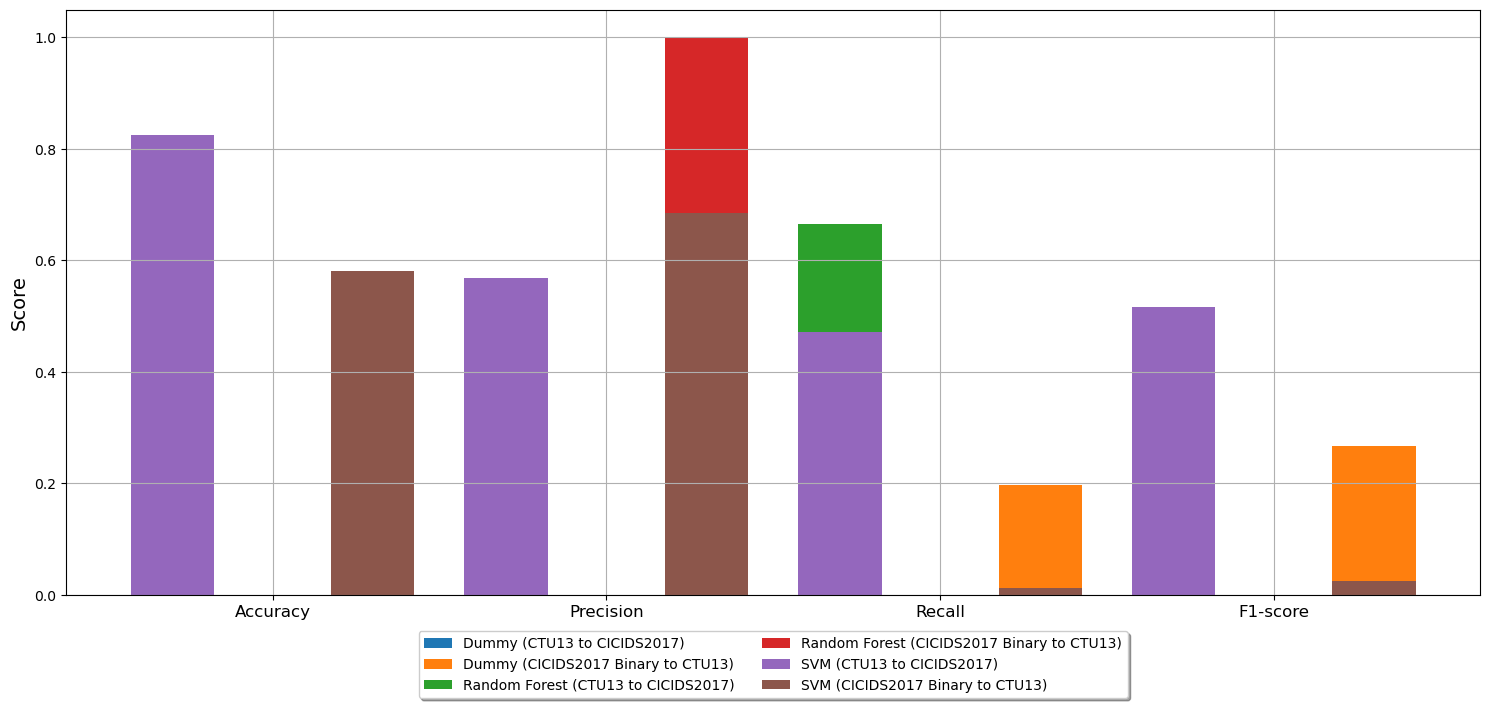
\includegraphics[width=1\textwidth]{img/Classifier_Performance _Across_Datasets.png}
    \caption{Classifiers' Performance on across datasets.}\label{fig:classifier_performance_across_dataset}
\end{figure}

\section{Feature Importance Analysis}

\begin{figure}[H]
    \centering
    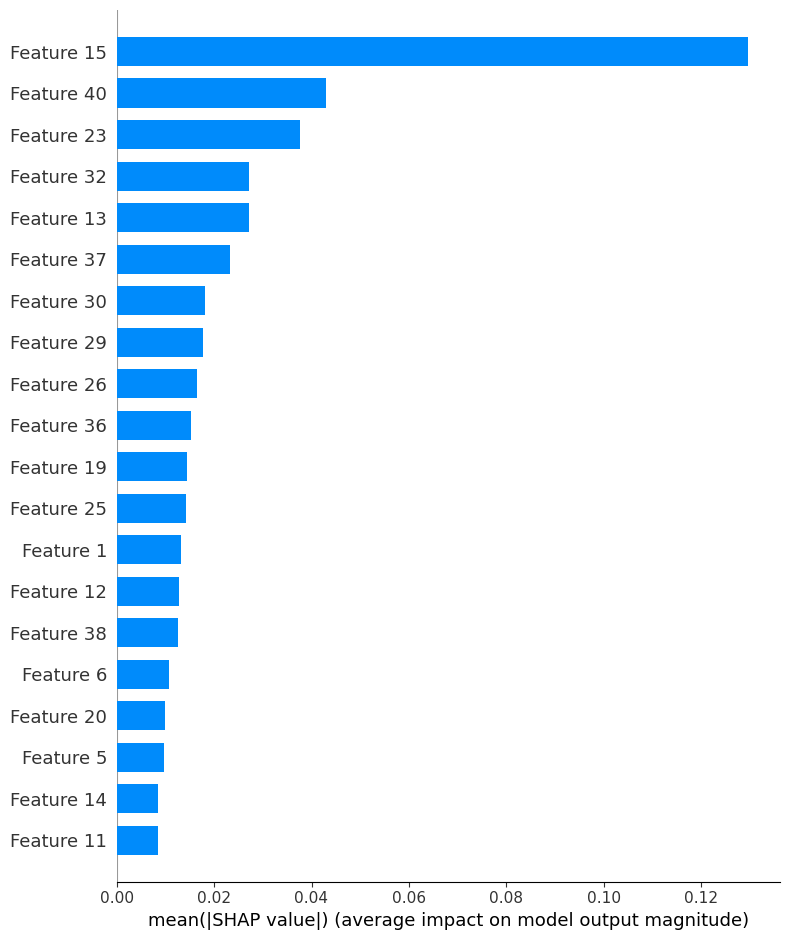
\includegraphics[width=1\textwidth]{img/SHAP_RFCTU13_CTU13.png}
    \caption{SHAP summary plot for the CTU13 random forest model tested against CTU13.}\label{fig:shap_rfc_ctu13_ctu13}
\end{figure}

\begin{figure}[H]
    \centering
    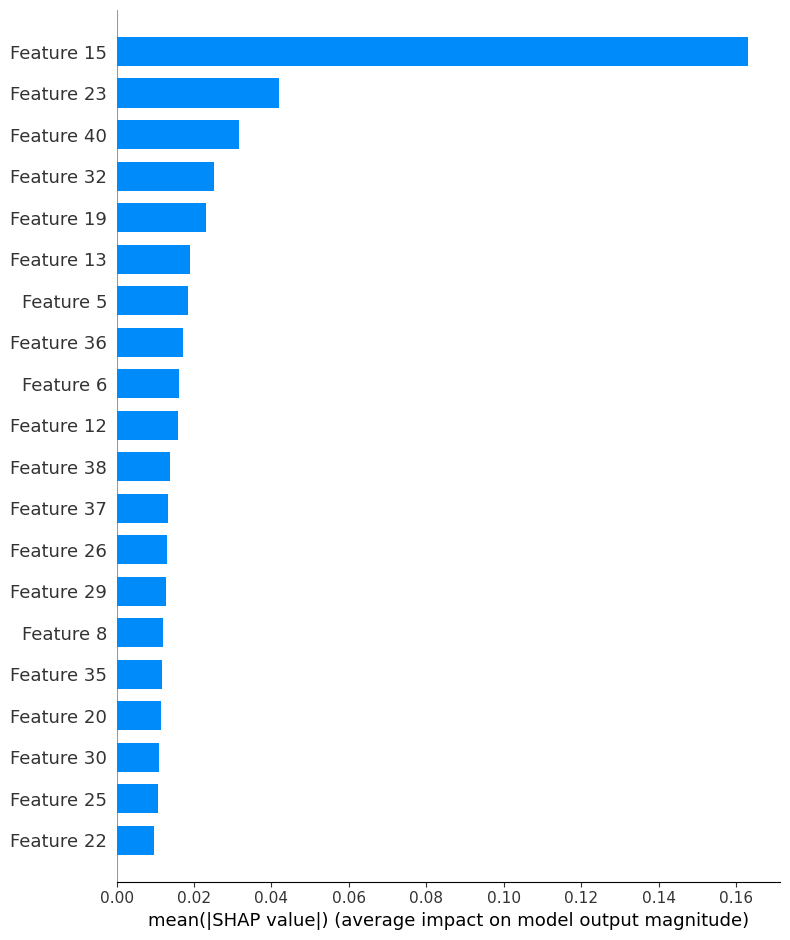
\includegraphics[width=1\textwidth]{img/SHAP_RFCTU13_CICIDS2017.png}
    \caption{SHAP summary plot for the CTU13 random forest model tested against CICIDS2017.}\label{fig:shap_rfc_ctu13_cicids2017}
\end{figure}

\begin{figure}[H]
    \centering
    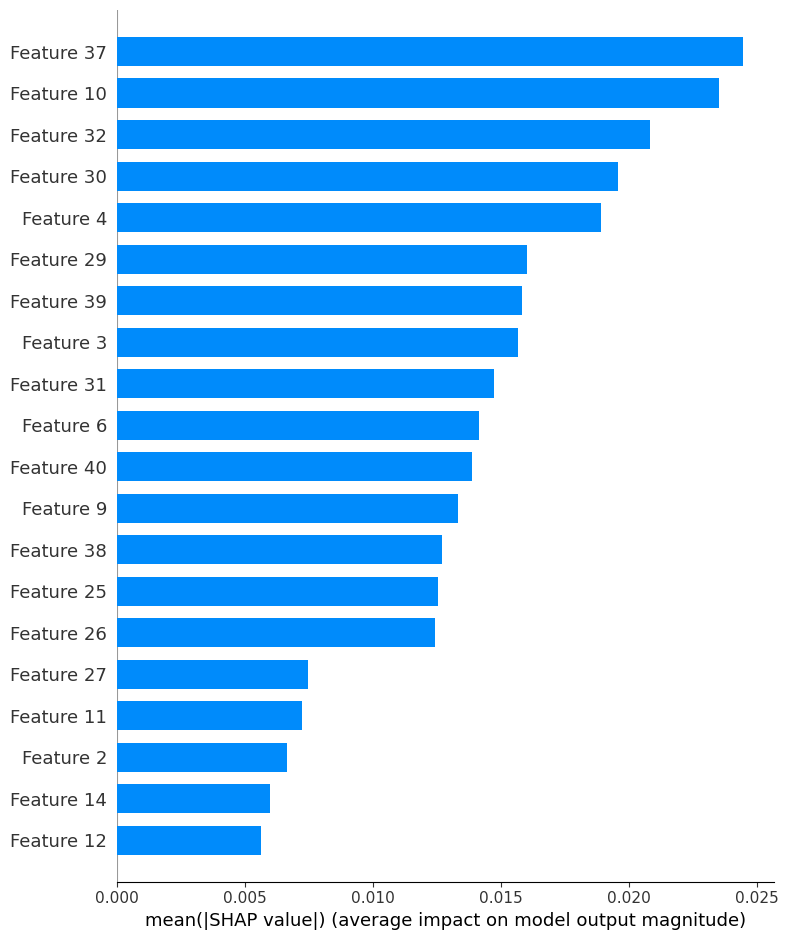
\includegraphics[width=1\textwidth]{img/SHAP_RFCICIDS2017_CICIDS2017.png}
    \caption{SHAP summary plot for the CICIDS2017 random forest model tested against CICIDS2017.}\label{fig:shap_rfc_cicids2017_cicids2017}
\end{figure}

\begin{figure}[H]
    \centering
    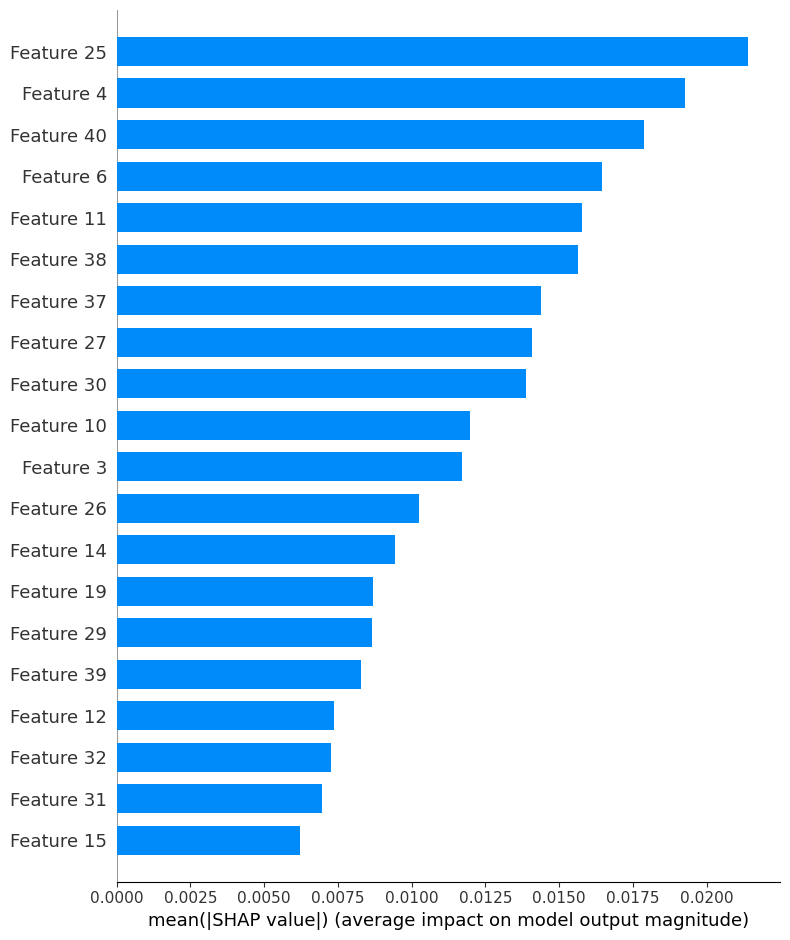
\includegraphics[width=1\textwidth]{img/SHAP_RFCICIDS2017_CTU13.png}
    \caption{SHAP summary plot for the CICIDS2017 random forest model tested against CTU13.}\label{fig:shap_rfc_cicids2017_ctu13}
\end{figure}

We analyse the SHAP (SHapley Additive exPlanations) values to identify the most influential features in the random forest classifiers' decisions. Figure~\ref{fig:shap_rfc_ctu13_ctu13} shows that when we test the CTU13 model on CTU13 data, features like Bwd Packet Length Mean and Flow IAT Min are important. However, when applied to CICIDS2017 (Figure~\ref{fig:shap_rfc_ctu13_cicids2017}), the model relies more on features like Flow Duration and Flow IAT Max, indicating a shift in feature importance when transferring to a new dataset.

The CICIDS2017 model tested on its data (Figure~\ref{fig:shap_rfc_cicids2017_cicids2017}) attributes importance to Fwd Packet Length Max and Average Packet Size. However, when evaluated on CTU13 (Figure~\ref{fig:shap_rfc_cicids2017_ctu13}), the model gives more weight to Fwd Header Length and Flow Duration. These variations in feature importance underscore the challenges in directly transferring models between datasets and the need for adaptive strategies.